\documentclass[a4paper]{article}
\usepackage{longtable}
\usepackage{graphicx}
\usepackage{lipsum}
\usepackage{hyperref}
\usepackage[style=numeric-comp,useprefix,hyperref,backend=bibtex]{biblatex}
\graphicspath{{../img/}}
\usepackage{endnotes}
\title{Wine Project Report}
\author{Ruggero Nocera (SXXXXXX) \\ Quarta Matteo (SXXXXXX)}
\date{}
\begin{document}

\maketitle
\tableofcontents

\section{Preliminary Data Analysis}
\lipsum[1]

\begin{center}
{\centering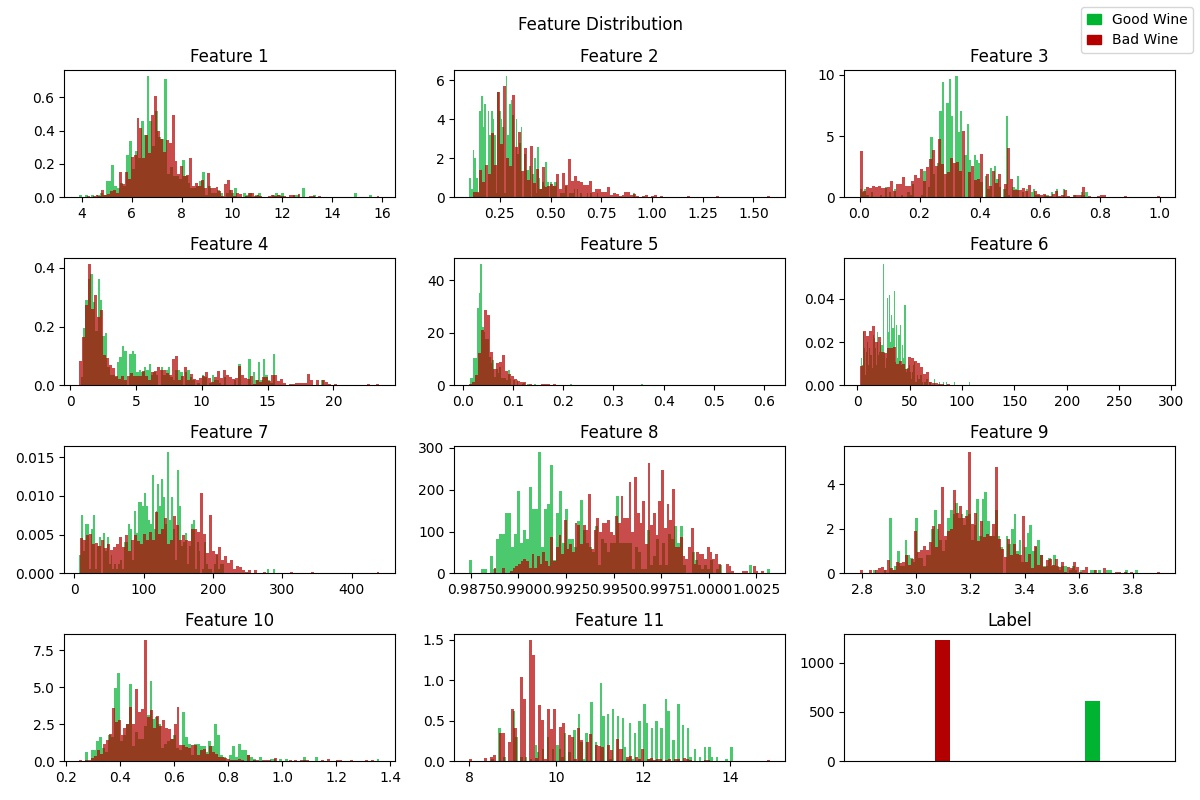
\includegraphics[width=\textwidth]{dist.jpg}}
\end{center}

\lipsum[2]
{\centering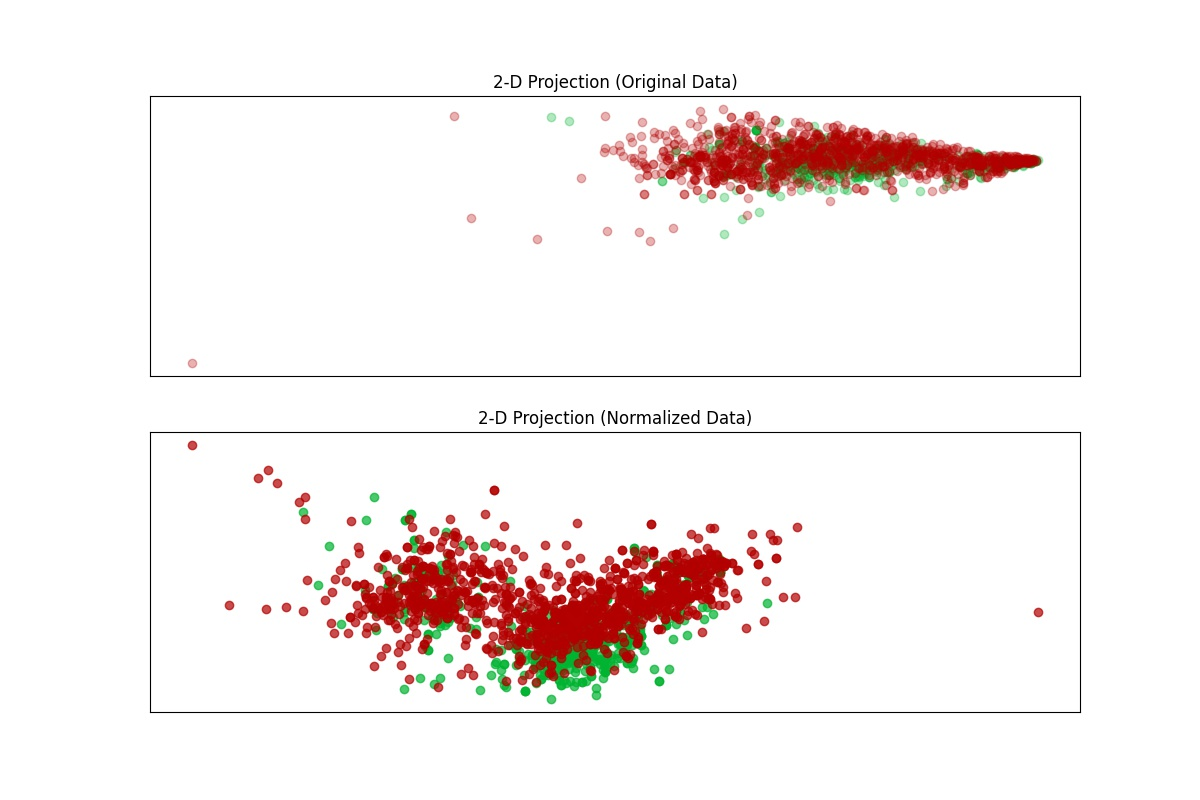
\includegraphics[width=\textwidth]{scatter.jpg}}

% Gaussian Cliassifiers Reulsts, put in a sep file??
\newpage
\begin{table}[!htb]
\centering
\begin{center}
\begin{longtable}{|c|c|c|}
\caption{MVG}\label{tab:mvg_acctable}\\
\hline
$\pi_T$ & PCA & Error Rate\\
\hline
\hline
\end{longtable}
\end{center}


\begin{center}
\begin{longtable}{|c|c|c|}
\caption{Naive Bayes}\label{tab:mvg_naiveacctable}\\
\hline
$\pi_T$ & PCA & Error Rate\\
\hline
0.5 & 6 & 19.978\% \\
\hline
0.6 & 10 & 19.539\% \\
\hline
0.6 & 9 & 18.496\% \\
\hline
0.6 & 8 & 18.825\% \\
\hline
0.6 & 7 & 18.332\% \\
\hline
0.6 & 6 & 18.880\% \\
\hline
0.6 & 5 & 18.771\% \\
\hline
0.7 & 10 & 17.838\% \\
\hline
0.7 & 9 & 18.277\% \\
\hline
0.7 & 8 & 17.124\% \\
\hline
0.7 & 7 & 17.783\% \\
\hline
0.7 & 6 & 18.716\% \\
\hline
0.7 & 5 & 18.716\% \\
\hline
0.8 & 10 & 17.508\% \\
\hline
0.8 & 9 & 17.563\% \\
\hline
0.8 & 8 & 18.277\% \\
\hline
0.8 & 7 & 18.222\% \\
\hline
0.8 & 6 & 19.265\% \\
\hline
0.8 & 5 & 19.429\% \\
\hline
0.9 & 10 & 18.332\% \\
\hline
0.9 & 9 & 19.704\% \\
\hline
\hline
\end{longtable}
\end{center}


\begin{center}
\begin{longtable}{|c|c|c|}
\caption{Tied Covariance}\label{tab:mvg_tiedcov}\\
\hline
$\pi_T$ & PCA & Error Rate\\
\hline
\hline
\end{longtable}
\end{center}

\end{table}


% Normalize Gaussian, put in a sep file??
\newpage
\begin{table}[!htb]
\begin{tabular}{|c|c|c|c|}
\hline
$\pi_T$ & PCA & Error Rate & $DCF_{norm}$\\
\hline
0.5 & 10 & 20.198\% & 0.404\\
\hline
0.5 & 8 & 20.527\% & 0.411\\
\hline
0.5 & 7 & 20.527\% & 0.411\\
\hline
0.5 & 9 & 20.637\% & 0.413\\
\hline
0.5 & 5 & 21.515\% & 0.430\\
\hline
0.5 & 6 & 21.734\% & 0.435\\
\hline
0.6 & 7 & 17.947\% & 0.449\\
\hline
0.6 & 10 & 18.441\% & 0.461\\
\hline
0.6 & 9 & 18.551\% & 0.464\\
\hline
0.6 & 8 & 18.551\% & 0.464\\
\hline
\end{tabular}
\caption{MVG (Normalized Samples)}\label{tab:mvgn_acctable}


\begin{tabular}{|c|c|c|c|}
\hline
$\pi_T$ & PCA & Error Rate & $DCF_{norm}$\\
\hline
0.5 & 7 & 20.472\% & 0.409\\
\hline
0.5 & 6 & 20.966\% & 0.419\\
\hline
0.5 & 8 & 21.131\% & 0.423\\
\hline
0.5 & 9 & 21.405\% & 0.428\\
\hline
0.5 & 5 & 21.734\% & 0.435\\
\hline
0.5 & 10 & 21.899\% & 0.438\\
\hline
0.5 & 4 & 23.381\% & 0.468\\
\hline
0.6 & 8 & 18.880\% & 0.472\\
\hline
0.6 & 9 & 19.649\% & 0.491\\
\hline
0.5 & 3 & 24.698\% & 0.494\\
\hline
\end{tabular}
\caption{Naive Bayes MVG (Normalized Samples)}\label{tab:mvgn_naiveacctable}


\caption{Tied Covariance MVG (Normalized Samples)}\label{tab:mvgn_tiedcov}
\begin{center}
\begin{tabular}{|c|c||c|c|}
\hline
\ & PCA & Error Rate & $DCF$\\
\hline
$\pi_T = 0.33$ & 11 & 18.05 & 0.547 \\
$\pi_T = 0.50$ & 11 & 16.86 & 0.337 \\
$\pi_T = 0.67$ & 11 & 27.30 & 0.827 \\
\hline
$\pi_T = 0.33$ & 9 & 18.43 & 0.559 \\
$\pi_T = 0.50$ & 9 & 16.91 & 0.338 \\
$\pi_T = 0.67$ & 9 & 27.35 & 0.829 \\
\hline
$\pi_T = 0.33$ & 10 & 18.49 & 0.560 \\
$\pi_T = 0.50$ & 10 & 17.02 & 0.340 \\
$\pi_T = 0.67$ & 10 & 27.30 & 0.827 \\
\hline
\end{tabular}
\end{center}



\end{table}


% Kernel RBF Results, put in a sep file??
\newpage
\begin{table}[!htb]
\centering
    \begin{center}
\begin{longtable}{|c|c|c|c|}
\caption{Kernel SVM}\label{tab:svm_rbf_acctable}\\
\hline
Bias & $\gamma$ & $C$ & Error Rate \\
\hline
0 & 5 & 0.1 & 27.168\% \\
\hline
0 & 5 & 1.0 & 27.168\% \\
\hline
0 & 10 & 0.1 & 27.442\% \\
\hline
0 & 10 & 1.0 & 27.442\% \\
\hline
1.0 & 5 & 0.1 & 36.443\% \\
\hline
1.0 & 5 & 1.0 & 36.443\% \\
\hline
1.0 & 10 & 0.1 & 36.443\% \\
\hline
1.0 & 10 & 1.0 & 36.443\% \\
\hline
\hline
\end{longtable}
\end{center}


    \begin{center}
\begin{tabular}{|c|c|c|c|c|}
\hline
Bias & $\gamma$ & $C$ & PCA & Error Rate \\
\hline
0 & 5 & 0.1 & 10 & 27.168\% \\
\hline
0 & 5 & 0.1 & 9 & 27.168\% \\
\hline
0 & 5 & 0.1 & 8 & 27.168\% \\
\hline
0 & 5 & 1 & 8 & 27.168\% \\
\hline
0 & 5 & 1 & 10 & 27.223\% \\
\hline
0 & 5 & 1 & 9 & 27.223\% \\
\hline
0 & 10 & 0.1 & 8 & 27.387\% \\
\hline
0 & 10 & 1 & 8 & 27.387\% \\
\hline
0 & 10 & 0.1 & 10 & 27.442\% \\
\hline
0 & 10 & 0.1 & 9 & 27.442\% \\
\hline
\end{tabular}
\end{center}
\caption{Kernel SVM With PCA}\label{tab:svm_rbfpca_acctable}


    \begin{center}
\begin{longtable}{|c|c|c|c|c|}
\caption{Kernel SVM With PCA and Z-Normalization}\label{tab:svm_rbfpcan_acctable}\\
\hline
Bias & $\gamma$ & $C$ & PCA & Error Rate \\
\hline
0 & 0.3 & 1 & 9 & 13.172\% \\
\hline
0 & 0.5 & 0.5 & 9 & 13.172\% \\
\hline
0 & 0.3 & 1 & 8 & 13.282\% \\
\hline
0 & 0.5 & 1 & 9 & 13.282\% \\
\hline
0.1 & 0.3 & 1 & 8 & 13.337\% \\
\hline
0.1 & 0.5 & 1 & 9 & 13.337\% \\
\hline
0 & 0.3 & 0.5 & 9 & 13.447\% \\
\hline
0 & 0.3 & 1 & 10 & 13.447\% \\
\hline
0 & 0.5 & 1 & 10 & 13.502\% \\
\hline
0 & 0.1 & 1 & 9 & 13.557\% \\
\hline
\end{longtable}
\end{center}

\end{table}

\end{document}